\documentclass{article}
\usepackage{subfigure}
\usepackage{graphicx}
\begin{document}


\begin{figure}[htbp]
    \centering  %居中
    \subfigure[500s后结果]{   %第一张子图
    \begin{minipage}{0.4\textwidth}%大小总和超过textwidth则自动换行
    \centering    %子图居中
    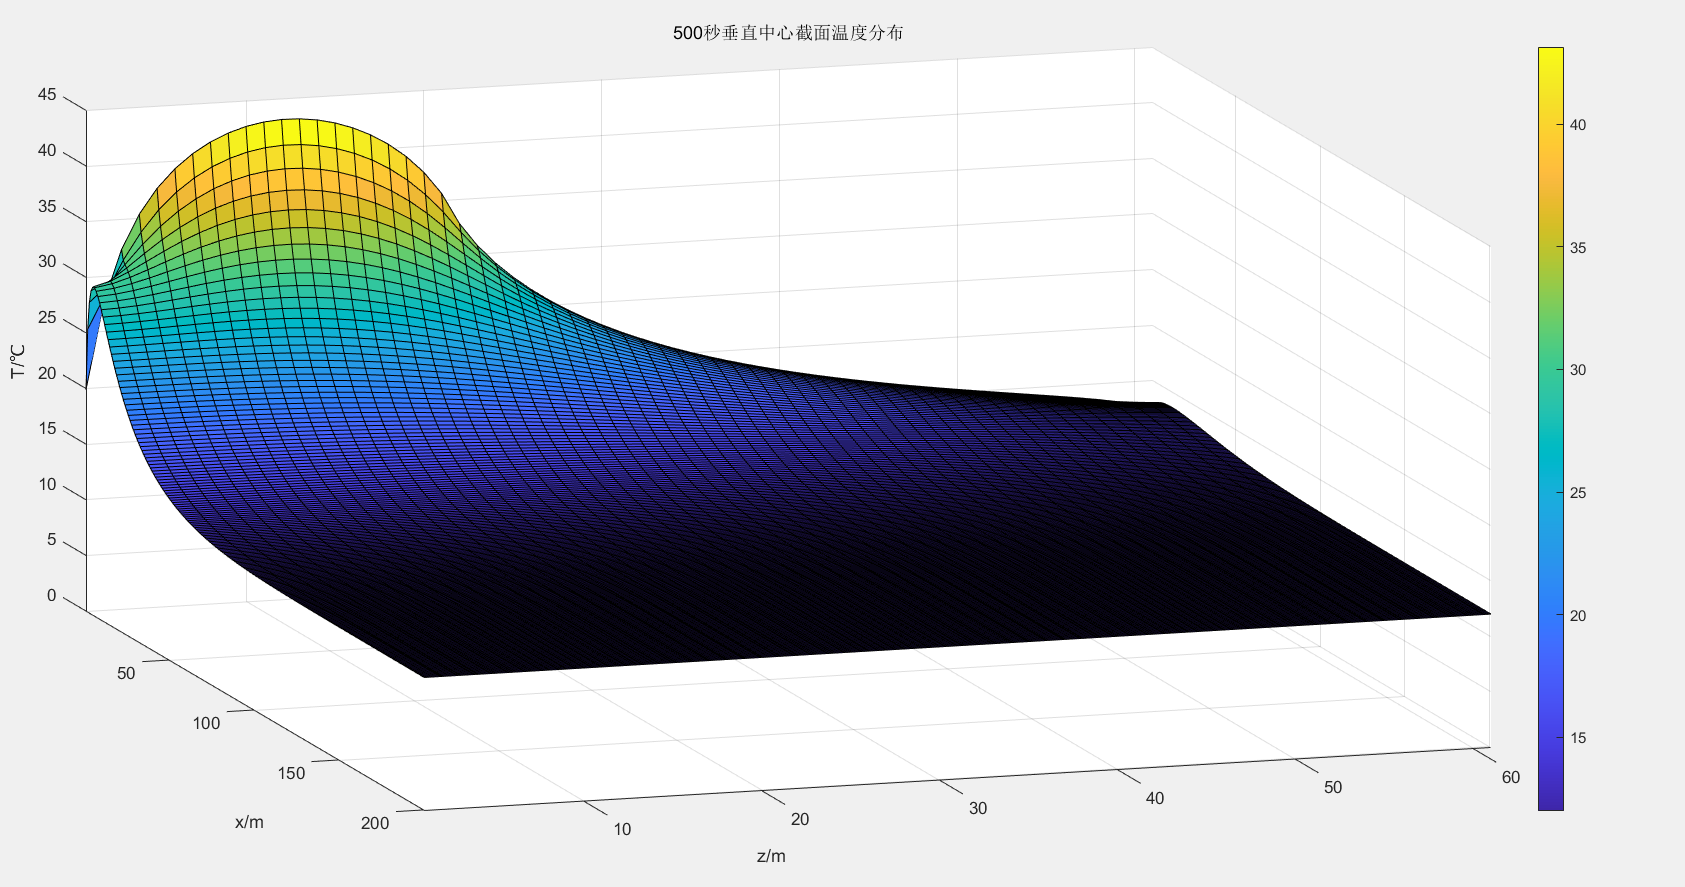
\includegraphics[width=\textwidth]{3d3.png}  %设置图片的输出大小倍数,这里是0.5倍大小输出
    \end{minipage}
    }
    \subfigure[122s后结果]{ %第二张子图
    \begin{minipage}{0.4\textwidth}
    \centering    %子图居中
    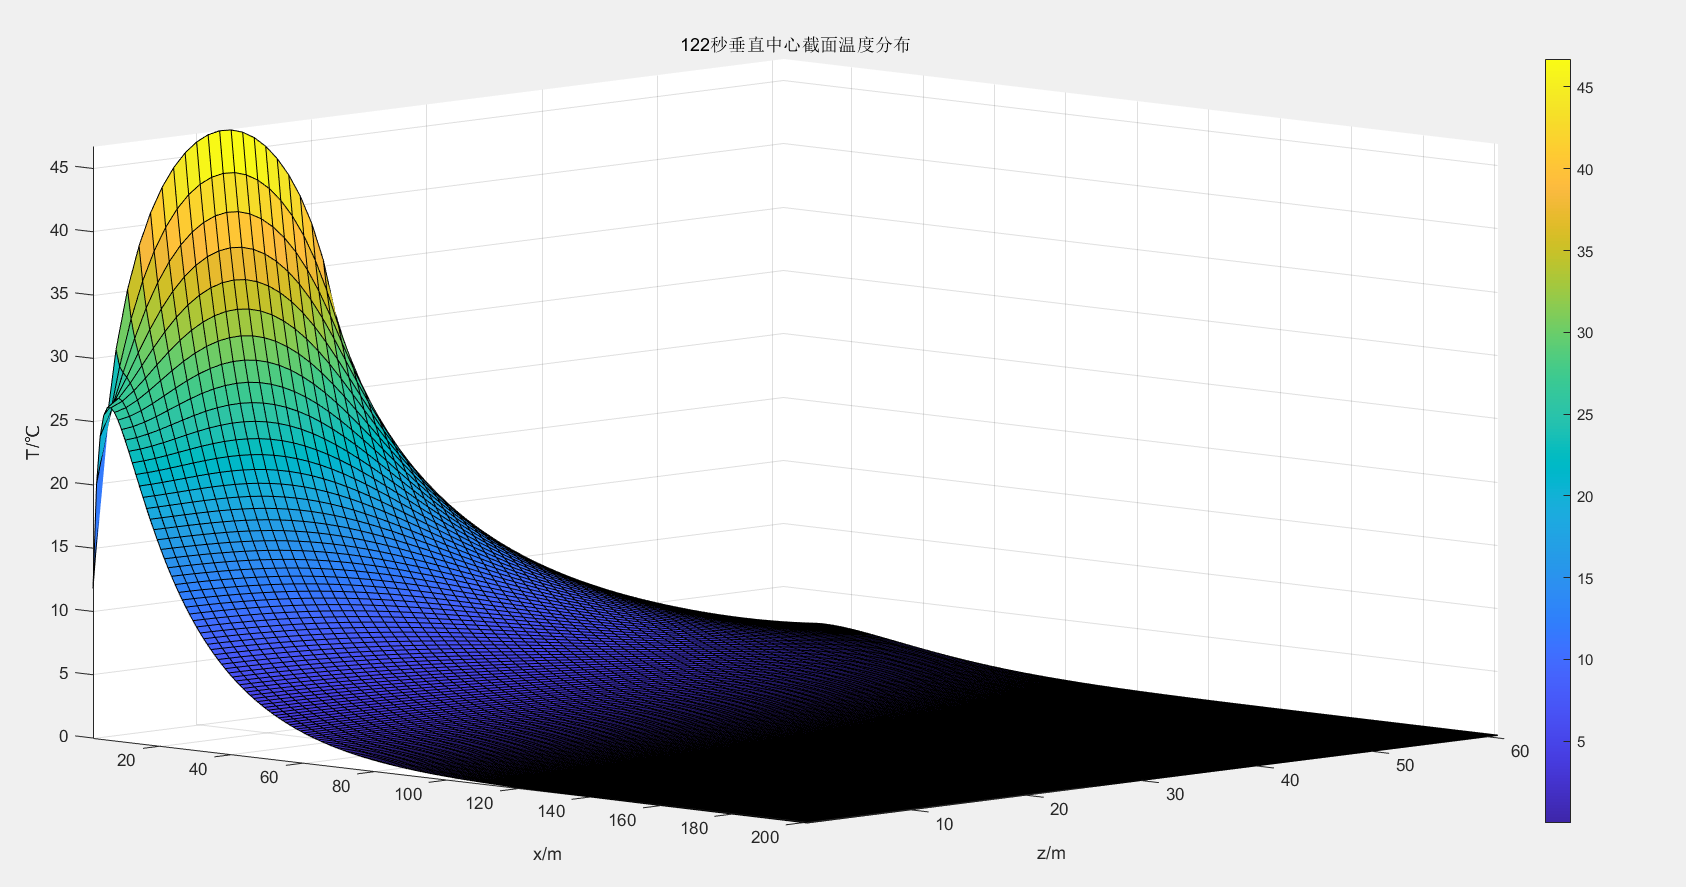
\includegraphics[width=\textwidth]{3d4.png}%以pic.jpg的0.5倍大小输出
    \end{minipage}
    }
    \caption{房屋温度在x-z方向上的截面图}    %大图名称
    \label{3d2}    %图片引用标记
\end{figure}

\end{document}